\chapter{Optimization Under Uncertainty}

\section{Robust Optimization}
Robust optimization deals with problems of decision-making under uncertainty, particularly focusing on creating solutions that remain feasible under all variations within specified uncertainty sets. This section introduces two prevalent forms of uncertainty: interval uncertainty for individual coefficients and ellipsoidal uncertainty for rows of a coefficient matrix.

\subsection{Interval Uncertainty}
In interval uncertainty, each coefficient in the data matrix or vector is assumed to have an upper and lower bound, representing the range of its possible values. For a linear programming problem, this can be written as:

\begin{equation}
\begin{aligned}
& \underset{x}{\text{minimize}}
& & c^T x \\
& \text{subject to}
& & A x \leq b, & \text{ for all } A \in [\underline{A}, \overline{A}], b \in [\underline{b}, \overline{b}]
\end{aligned}
\end{equation}

where \(x\) is the vector of decision variables, \(c\) is the cost vector, \(A\) and \(b\) are the technology matrix and resource vector with their respective ranges defined by the lower \(\underline{A}, \underline{b}\) and upper \(\overline{A}, \overline{b}\) bounds. 
\begin{center}
\begin{tikzpicture}
  % Draw the number line
  \draw[latex-latex] (0,0) -- (10,0); 
  % Place the interval endpoints
  \draw[thick] (3,-0.1) -- (3,0.1) node[above] {$\underline{A_{ij}}$};
  \draw[thick] (7,-0.1) -- (7,0.1) node[above] {$\overline{A_{ij}}$};
  % Place the coefficient A_ij
  \node[draw,circle,inner sep=2pt,fill=black,label=above:{$A_{ij}$}] at (5,0) {};
  % Add dashed lines to denote the range
  \draw[dashed] (3,0) -- (3,-0.75);
  \draw[dashed] (7,0) -- (7,-0.75);
  \draw[<->] (3,-0.5) -- (7,-0.5) node[midway,below] {Range of $A_{ij}$};
\end{tikzpicture}
\end{center}

\begin{example}{Interval Uncertainty in LP}{}
Consider the LP problem
\begin{equation}
\begin{aligned}
& \underset{x}{\text{minimize}}
& & 2x_1 - 3x_2 \\
& \text{subject to}
& & x_1 + 2x_2 \leq 3, \\
&&& 3x_1 + x_2 \leq 2, \\
&&& x_1, x_2 \geq 0,
\end{aligned}
\end{equation}
but now we assume that the coefficients in the LP might be uncertain up to 10\%.  

For the objective function, coefficients of \( x_1 \) and \( x_2 \) are within intervals [1.8, 2.2] and [-3.3, -2.7], respectively.\\
 The constraint coefficients are within the following intervals: for the first constraint, \( x_1 \) is in [0.9, 1.1] and \( x_2 \) is in [1.8, 2.2]; for the second constraint, \( x_1 \) is in [2.7, 3.3] and \( x_2 \) is in [0.9, 1.1]. The bounds on \( b \) are the constant terms on the right side of the constraints, which are assumed to be fixed for this example.

The LP formulation considering the worst-case scenario for the coefficient intervals is as follows:
\begin{equation}
\begin{aligned}
& \underset{x}{\text{minimize}}
& & 2.2x_1 - 2.7x_2 \\
& \text{subject to}
& & 1.1x_1 + 2.2x_2 \leq 3, \\
&&& 3.3x_1 + 1.1x_2 \leq 2, \\
&&& x_1, x_2 \geq 0.
\end{aligned}
\end{equation}

This LP takes the upper bound of coefficients for the objective function and the lower bound for the constraints, thereby presenting the most conservative estimate of the solution space in face of the given uncertainties.

\begin{center}
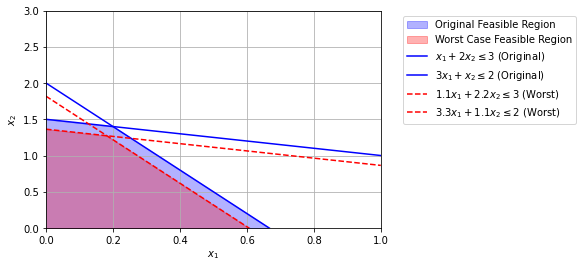
\includegraphics[scale = 0.4]{robust-feasible-region}
\end{center}
\end{example}

\subsection{Ellipsoidal Uncertainty - Stolen From Boyd Convex Optimization}
Ellipsoidal uncertainty models the uncertainty in a row \(a^i\) of the matrix \(A\) as lying within an ellipsoid or ball. The uncertain row \(a^i\) can be represented as:

\begin{equation}
a^i \in \mathcal E_i := \{\bar a^i + U^id \ : \  \|d\|_2 \leq 1\},
\end{equation}
where \(\bar a^i\) is the nominal row vector, \(U^i\) is a matrix specifying the directions of deviation for row \(i\), \(d\) is a deviation vector within the unit ball. 

\begin{center}
\begin{tikzpicture}[scale=1.5, every node/.style={scale=1.5}]
  % Draw the ellipsoid using an ellipse shape
  \draw[fill = yellow, opacity = 0.3] (0,0) ellipse (3cm and 1.5cm);
  
  % Draw vector a^i as an arrow from origin
  \draw[-{Latex[length=3mm,width=2mm]}] (0,0) -- (1.5,0.5) node[midway, above] {$U^id$};

  % Optional: Add the center point of the ellipsoid if needed
  \filldraw (0,0) circle (1pt) node[below left] {$\bar a^i$};
  \filldraw (1.5,0.5) circle (1pt) node[right] {$a^i$};

  % Label the ellipsoid
  %\node at (3.3,-1) {Ellipsoid};

  % Optional: Add coordinate grid for reference if desired
  %\draw[step=0.5cm,gray,very thin] (-3,-2) grid (3,2);

\end{tikzpicture}
\end{center}

Robust linear programming
We consider a linear program in inequality form,
$$
\begin{array}{ll}
\operatorname{minimize} & c^T x \\
\text { subject to } & a_i^T x \leq b_i, \quad i=1, \ldots, m
\end{array}
$$
in which there is some uncertainty or variation in the parameters $c, a_i, b_i$. To simplify the exposition we assume that $c$ and $b_i$ are fixed, and that $a_i$ are known to lie in given ellipsoids:
$$
a_i \in \mathcal{E}_i=\left\{\bar{a}_i+P_i u \mid\|u\|_2 \leq 1\right\}
$$
where $P_i \in \mathbf{R}^{n \times n}$. (If $P_i$ is singular we obtain 'flat' ellipsoids, of dimension rank $P_i$; $P_i=0$ means that $a_i$ is known perfectly.)

We will require that the constraints be satisfied for all possible values of the parameters $a_i$, which leads us to the robust linear program
$$
\begin{array}{ll}
\operatorname{minimize} & c^T x \\
\text { subject to } & a_i^T x \leq b_i \text { for all } a_i \in \mathcal{E}_i, \quad i=1, \ldots, m .
\end{array}
$$

The robust linear constraint, $a_i^T x \leq b_i$ for all $a_i \in \mathcal{E}_i$, can be expressed as
$$
\sup \left\{a_i^T x \mid a_i \in \mathcal{E}_i\right\} \leq b_i
$$
the lefthand side of which can be expressed as
$$
\begin{aligned}
\sup \left\{a_i^T x \mid a_i \in \mathcal{E}_i\right\} & =\bar{a}_i^T x+\sup \left\{u^T P_i^T x \mid\|u\|_2 \leq 1\right\} \\
& =\bar{a}_i^T x+\left\|P_i^T x\right\|_2
\end{aligned}
$$

Thus, the robust linear constraint can be expressed as
$$
\bar{a}_i^T x+\left\|P_i^T x\right\|_2 \leq b_i,
$$
which is evidently a second-order cone constraint. Hence the robust LP (4.37) can be expressed as the SOCP
$$
\begin{array}{ll}
\operatorname{minimize} & c^T x \\
\text { subject to } & \bar{a}_i^T x+\left\|P_i^T x\right\|_2 \leq b_i, \quad i=1, \ldots, m
\end{array}
$$

Note that the additional norm terms act as regularization terms; they prevent $x$ from being large in directions with considerable uncertainty in the parameters $a_i$.


%This SOCP formulation ensures that the constraint holds for all \(a\) within the specified ellipsoid. Here, \(\delta \| U^T x \|_2\) represents the worst-case additive term due to uncertainty in \(a\), ensuring that the solution \(x\) is feasible under all possible realizations of \(a\).

